\section{Case Study}
\subsection{MNIST}
The neuromorphic network designed earlier on is applied to computer vision application of MNIST (Figure \ref{fig:mnist}) dataset. This dataset has 60000 samples available for training and 10000 samples available for testing. For training wise, TensorFlow python library and Keras framework were used. For computer vision prediction result visualisation as shown in Figure \ref{fig:predict}, OpenCV library was deployed. These libraries and framework is briefly described in Table \ref{tbl:tooloftrade}. Their description are adapted from their official websites.
\begin{figure}[H]
	\centering
	\includegraphics[scale=1]{mnist.png}
	\caption{ Modified National Institute of Standards and Technology (MNIST) Handwritten digit database}
	\label{fig:mnist}
\end{figure}
\begin{table}[ht]
	\centering
	\begin{tabular}[t]{cL{11cm}}
		\hline
		Tools & Description\\
		\hline
		\hline
		TensorFlow & Google's open source library for machine learning training and development. \cite{tensorflow}\\
		Keras & TensorFlow's high-level application interface for deep learning models developments. It's used for fast prototyping, state-of-the-art research, and production. \cite{keras}\\
		OpenCV & Open Source Computer Vision Library (OpenCV) is an open source computer vision and machine learning software library. OpenCV provides a common infrastructure for computer vision applications and speeds up the commercial use of machine perception. \cite{opencv}\\
		\hline
	\end{tabular}
	\caption{Table of tools of trade}
	\label{tbl:tooloftrade}
\end{table}
As discussed before, each neuron output is fed to an activation function like shown in Figure \ref{fig:relu} and Figure \ref{fig:sigmoid}. Without an activation function, our network is just a linear regression model. That is, its continuous output is as a result of linear function. Linear functions cannot properly fit complex non-linear dataset. Therefore, we need these non-linear activation function as follows. Although ReLU looks like linear activation function, it is in fact non-linear due to changing gradient at $x=0$. For softmax activation function, let say we have 3 neuron with output $a$, $b$ and $c$ respectively. the final output of neuron 1, 2, and 3 would be $\frac{e^a}{e^a + e^b + e^c}$, $\frac{e^b}{e^a + e^b + e^c}$ and $\frac{e^c}{e^a + e^b + e^c}$ respectively.
\begin{figure}[H]
	\centering
	\includegraphics[scale=0.7]{relu.png}
	\caption{Rectified linear unit (ReLU) activation function}
	\label{fig:relu}
\end{figure}
\begin{figure}[H]
	\centering
	\includegraphics[scale=0.7]{sigmoid.png}
	\caption{Sigmoid function, a special case of Softmax activation function with 2 outputs and one output set to 0}
	\label{fig:sigmoid}
\end{figure}
A few network architecture has been attempted to test the performance of previous activation function (Table \ref{tbl:netarc}). FCN 100 here means fully connected network, i.e. all input neurons in input layer connect to each of the 100 neuron in the hidden layer. The table shows ReLU activation function is meant for hidden layers with softmax function meant for output layer.
\begin{table}[ht]
	\centering
	\begin{tabular}[t]{L{11cm}c}
		\hline
		Network Architecture & Accuracy\\
		\hline
		\hline
		Input $\rightarrow$ FCN 100 $\rightarrow$ output
		& 11.78\%\\
		Input $\rightarrow$ FCN 100 with ReLU activation $\rightarrow$ output
		& 11.35\%\\
		Input $\rightarrow$ FCN 100 with ReLU activation $\rightarrow$ output with ReLU activation
		& 9.8\%\\
		\rowcolor{lg} Input $\rightarrow$ FCN 100 with ReLU activation $\rightarrow$ output with softmax activation
		& 96.91\%\\
		Input $\rightarrow$ FCN 100 with softmax activation $\rightarrow$ output with softmax activation
		& 54.97\%\\
		\hline
	\end{tabular}
	\caption{Table of network architecture with different activation function variation and their accuracies (highest accuracy is highlighted in green)}
	\label{tbl:netarc}
\end{table}
Techniques such as maxpooling (Figure \ref{fig:maxpool}) and 2D convolution (Figure \ref{fig:conv2d}) are used. Maxpooling reduces matrix to smaller size with only the largest values. Furthermore, multi layers of convolution matrix being used to extract different features, i.e. curvature, strokes and etc. It is achieved by summing the multiplication of individual elements between large data matrix and small convolution matrix of the overlapped region. For these 2 techniques, we have a small matrix sliding across a large data matrix to perform operation. Visually, it means sliding from left to right, from ${\text{1}}^{\text{st}}$ on top to last row at the bottom. The sliding motion is in a form of 1 step or few steps at once. For maxpooling, the sliding step size is 2, whereas for 2D convolution matrix the sliding step size is 1.
\begin{figure}[H]
	\centering
	\includegraphics[scale=0.5]{maxpool.png}
	\caption{Maxpooling}
	\label{fig:maxpool}
\end{figure}
\begin{figure}[H]
	\subfloat[2D convolution at the start
	]{
		\centering
		\includegraphics[scale=0.45]{conv1.png}
	}
	\subfloat[2D convolution at the end]{
		\centering
		\includegraphics[scale=0.45]{conv2.png}    
	}
	\caption{2D convolution operation}
	\label{fig:conv2d}
\end{figure}
Unlike the architecture of Table \ref{tbl:netarc}, a higher performing one involves more than just FCN. It consists of multiple repetitive units of 2D convolution, followed by maxpooling, before it is flatten from 2D matrixes to 1D vector, and finally reaching the FCN and output layer (See Figure \ref{fig:cnnseq}). Each deeper repetitive unit of 2D convolution and maxpooling extracts subtler features. Let's look at the 2 repetitive units in greater detail. An output of convolution layer is known as feature map. If we have $n1$ convolution matrixes working on a 2D input, there will be $n1$ feature maps, which look like a 3D stack. These feature maps will go through maxpooling to reduce the its 2D dimension, retaining its 3D height. The next convolution layer that has $n2$ convolution matrixes will have each of its matrices working on the 3D stack individually. The way it work on the 3D stack is a slightly modified version of Figure \ref{fig:conv2d}. In the figure, we have 1 matrix working on 1 feature map of the previous repetitive unit. Now, we have $n1$ feature map in a form of 3D stack, hence, the matrix will work on the intersected volume ($n1$ height), not just intersected area. Let's say the top most feature map matrix operation of top left area result is 4 as shown in Figure \ref{fig:conv2d}, the intersected lower layers we have value $a,b,c,...$, therefore the output (top left corner unit of a 2D feature map) will be $4+a+b+c+...$ ($n1$ terms of them). A complete operation yields a complete 2D feature map. Do note that this is just 1 2D feature map of the 3D matrix operation from 1 of the $n2$ matrices.  All $n2$ 3D matrix operations yield $n2$ layers of 3D feature map stack. Flattening will simply be extracting rows by rows of a 3D volume into a 1D vector. The rest of FCN network is already explained in subsection \ref{sect:ann}.
\begin{figure}[H]
	\centering
	\includegraphics[scale=0.3]{cnnsequence.jpeg}
	\caption{An example convolutional neural network sequence}
	\label {fig:cnnseq}
\end{figure}
A few types of network architecture have been attempted to discover the network characteristic by tuning the number of neuron in FCN, introducing convolutional layers, and varying the number of convolutional network matrices.
\begin{table}[ht]
	\centering
	\begin{tabular}[t]{cL{11cm}}
		\hline
		Abbreviated Title & Full Description\\
		\hline
		\hline
		$n$ FCN & Input Layer $\rightarrow$ Flattening Layer $\rightarrow$ $n$ Neurons Fully Connected Layer $\rightarrow$ 10 Neurons Fully Connected Layer $\rightarrow$ Softmax Activation Layer\\
		$n$ Conv Maxpool 10 FCN & Input Layer $\rightarrow$ $n$ 2D Convolutional Layers with $5\times 5$ Kernel Size $\rightarrow$ $n$ ReLU Activation Layers $\rightarrow$ $n$ 2D Max Pooling Layers with $2\times2$ Window Size \& 2 Strides $\rightarrow$ Flattening Layer $\rightarrow$ 10 Neurons Fully Connected Layer $\rightarrow$ Softmax Activation Layer\\
		(20 Conv Maxpool) $\times 2$ 10 FCN &  Input Layer $\rightarrow$ 20 2D Convolutional Layers with $5\times 5$ Kernel Size $\rightarrow$ 20 ReLU Activation Layers $\rightarrow$ 20 2D Max Pooling Layers with $2\times2$ Window Size \& 2 Strides $\rightarrow$ 20 2D Convolutional Layers with $5\times 5$ Kernel Size $\rightarrow$ 20 ReLU Activation Layers $\rightarrow$ 20 2D Max Pooling Layers with $2\times2$ Window Size \& 2 Strides $\rightarrow$ Flattening Layer $\rightarrow$ 10 Neurons Fully Connected Layer $\rightarrow$ Softmax Activation Layer\\
		20 Conv 50 Conv Maxpool 10 FCN & Input Layer $\rightarrow$ 20 2D Convolutional Layers with $5\times 5$ Kernel Size $\rightarrow$ 20 ReLU Activation Layers $\rightarrow$ 20 2D Max Pooling Layers with $2\times2$ Window Size \& 2 Strides $\rightarrow$ 50 2D Convolutional Layers with $5\times 5$ Kernel Size $\rightarrow$ 50 ReLU Activation Layers $\rightarrow$ 50 2D Max Pooling Layers with $2\times2$ Window Size \& 2 Strides $\rightarrow$ Flattening Layer $\rightarrow$ 10 Neurons Fully Connected Layer $\rightarrow$ Softmax Activation Layer\\
		\hline
	\end{tabular}
	\caption{Table of legends for TensorFlow trained graphs}
\end{table}

A few weight post processing function were used on trained weight in Tensorflow and Keras, to prepare our trained neural network for neuromorphic circuit weight transfer in Cadence. Following are the weight processing function name and their description:
\begin{enumerate}
	\item step:\\
	Originally, we have 
	discrete 8 steps $w_{c}$ in Table \ref{fig:rnw}. In Figure \ref{fig:scaledr}, we have $s$ ($x$ axis), a scale factor and the corresponding compressed weight value between upper bound and lower bound.  This is computed by $w_{c}/s$. There is no whatsoever compressing being done here although we talked about those compressed weight values as we are merely using them. With these 8 steps or 9 valued $w_{c}/s$, any input $w$ below the lower bound gets clipped to the lower bound value, whereas those above upper bound get clipped to upper value and those within the boundary get rounded to nearest $w_{c}/s$.
	\item stepUniform:\\
	Unlike previously where we used non-uniform values from Table \ref{fig:rnw}, we process the input directly. We assumed the input $w$ to be $0 \leq w \leq 1$, for given $n$ steps, or $n+1$ levels with uniform spacing, input $w$ is rounded to one of these $n+1$ levels that $w_{\text{processed}}$ is still $0 \leq w_{\text{processed}} \leq 1$. In the event our assumption of $0 \leq w \leq 1$ is false, where $w$ can be $>1$, $w$ is still rounded to one of the uniformly spaced $n+1$ levels with $w_{\text{processed}} > 1$.
	\item lim:\\
	Similar to ``step" function before, we still have the upper bound and lower bound with values from $w_c$ which set the clipping value in case our input $w$ exceeds them. The difference here is we have continuous, unprocessed, original input $w$ within the boundary, not rounded to nearest step values.
	\item compdecomp:\\
	There are actual compression and decompression done here. For example, we want to map $w$, a.k.a. $w_d$, within $[0,1]$ to $w_c$ within $[a,b]$ for compression, and vice versa for decompression, since decompression is just an inverse function of compression . We can derive the decompression function as follows:
	\begin{quote}
		For boundary value $w_c=b$, $\frac{b-a}{b-a}=1$ as needed.
		For boundary value $w_c=a$, we get $\frac{a-a}{b-a}=0$ as expected.
		Hence, the actual decompression function is:
		$$f(w_c) = \frac{w_c-a}{b-a}$$
		and compression function is:
		$$f(w_d) = w_d(b-a)+a$$
	\end{quote}
	For actual compression and decompression,
	$a$ and $b$ are $\frac{1}{3s}$ and $\frac{1}{s}$ respectively where $s$ is a scale factor like before.
	Steps taken to implement this function starts with compression to range $[\frac{1}{3s},\frac{1}{s}]$, ``step" function to round off to nearest $w_c$ level within the same range (see ``step" function), and finally decompression to scale back to range $[0,1]$.
\end{enumerate}
\begin{table}[H]
	\centering
	\begin{tabular}[t]{cL{9.8cm}c}
		\hline
		Figure & Figure Description & Weight Processing Function Used\\
		\hline
		\hline
		Figure \ref{fig:clipstep} & $0 \leq \text{weights} \leq 1$ (MRAM 8 steps non-uniform scaling with lossy rounding and capping) & step\\
		Figure \ref{fig:cliplim} & $0 \leq \text{weights} \leq 1$ (Continuous scaling with lossy capping) & lim\\
		Figure \ref{fig:clipuniform} & $0 \leq \text{weights}$ (Uniform scaling with $n$ steps lossy rounding) & stepUniform\\
		Figure \ref{fig:compdecomp} & $0 \leq \text{weights} \leq 1$ (MRAM 8 steps non-uniform lossy rounding with lossless compression/decompression) &  compdecomp\\
		Figure \ref{fig:lim} & $0 \leq \text{weights} \leq 1$ (Continuous scaling with lossy capping) & limit\\
		Figure \ref{fig:uniform} & $0 \leq \text{weights} \leq 1$ (Uniform scaling with $n$ steps lossy rounding) & stepUniform\\
		\hline
	\end{tabular}
	\caption{Table of figures and weight processing function used}
	\label{tbl:fignwproc}
\end{table}
Those 6 figures in Table \ref{tbl:fignwproc} were evaluated in the following pages. First 3 figures have their weights ranging $>1$ due to a false assumption of TensorFlow constraint in training that positive weight is never $>1$, whereas last 3 figures are all between 0 and 1. There are a few values, falling slightly to $\approx -0.1$ (See Figure \ref{fig:weightdist} and these values will be clipped) due to gradual implemention of constraint in training the network so as to achieve optimal learning rate as shown in Figure \ref{fig:lrate}. In general sense, factors that contribute significantly to low network performance are weight clipping and large size of network. The former limits the range of weight that can be represented and therefore distort the trained model (architecture + weight), whereas the latter amplifies the distortion when the network scales and complexity increases. Worst case for all the network accuracy is at around 10\%, i.e. the network gets 1/10 correct by getting stuck to a particular digit prediction for all 0-9 digits in uniform distribution. Clipping/Capping is very bad for weight value that fall outside the boundary. Where clipping has failed, weight compression and decompression comes to rescue by flat lining throughout (Figure \ref{fig:compdecomp}). The flat lining effect is due to the process compression and decompression is lossless and the only lossy process is rounding to nearest step. Nevertheless, the performance still drop for weight processed with ``compdecomp" due to larger network size (errors from rounding to nearest step and clipping of weight falling slightly below 0 got amplified). Other than 8 steps weight from MRAM, $n$ steps weight are also experimented so that we can get the optimal $n$ steps for future MRAM without sacrificing too much network performance. Those figures with uniform scaling (Figure \ref{fig:clipuniform} and Figure \ref{fig:uniform}) with $n$ steps converge to extremely high accuracy. Another phenomena we observed is a network performance is the lowest for highest scaled R due to a few important and influential (on the outcome) high weight $w$ got filtered out (outside the boundary), leaving many low weight $w$ lying around within the boundary, forming the model.

Finally, 20 FCN model (highlighted in green in Figure \ref{fig:compdecomp}) was chosen for its attributes such as very reasonably high accuracy of 80.24\% and significantly smaller scale and simpler implementation of network, minus away complex convolution and maxpooling function. These 2 functions are good in neural network, but they complicate simple neuromorphic network task of recognizing handwritten digits by demanding for more complex circuit, and asking for more errors.
\begin{figure}[H]
	\centering
	\includegraphics[scale=0.3]{weightdist.png}
	\caption{Original and modified (rounded) weight distribution for 20 FCN with ``compdecomp" weight processing function}
	\label{fig:weightdist}
\end{figure}
\begin{figure}[H]
	\centering
	\includegraphics[scale=0.3]{weightdistzoom.png}
	\caption{Figure \ref{fig:weightdist} (zoomed). Note those higher but sparser weight distribution towards the right.}
	\label{fig:weightdistzoom}
\end{figure}
In Figure \ref{fig:weightdist}, most weight cluster around 0, with some extending slightly before 0 as discussed earlier. These weight will be clipped to the leftmost modified weight at the extreme end of boundary (orange). It is quite lucky in a sense that the distribution of 8 steps modified weight of mram (orange) closely mimicks the distribution of weight (blue) due to its non linear spacing. By that it means, denser/tighter spacing of modified weight (orange) is observed towards the left end where the lower weight (blue) has the highest distribution towards the end (at 0, ignore those $<0$), and increasingly sparser spacing of modified weight (orange) towards the right where the higher/more influential weight (blue) has the lowest distribution (see zoomed Figure \ref{fig:weightdistzoom}).
\begin{figure}[H]
	\subfloat[10 FCN
	]{
		\centering
		\includegraphics[scale=0.55]{exceeds/input 10 dense step mram 17.40 max at 67.png}
	}
	\subfloat[1000 FCN]{
		\centering
		\includegraphics[scale=0.55]{exceeds/input 1000 dense step mram 14.49 max at 52.png}    
	}
	\\
	\subfloat[20 Conv Maxpool 10 FCN
	]{
		\centering
		\includegraphics[scale=0.55]{exceeds/input 20 conv maxpool 10 dense step mram 25.50 max at 35.png}
	}
	\subfloat[100 Conv Maxpool 10 FCN
	]{
		\centering
		\includegraphics[scale=0.55]{exceeds/input 100 conv maxpool 10 dense step mram 10.28 max at 1.png}    
	}
	\\
	\subfloat[(20 Conv Maxpool)$\times$2 10 FCN
	]{
		\centering
		\includegraphics[scale=0.55]{exceeds/input 20 conv maxpool x2 10 dense step mram 10.09 max at 1.png}
	}
	\subfloat[20 Conv Maxpool 50 Conv Maxpool 10 FCN]{
		\centering
		\includegraphics[scale=0.55]{exceeds/input 20 conv maxpool 50 conv maxpool 10 dense step mram 10.10 max at 1.png}    
	}
	\caption{$0 \leq \text{weights} \leq 1$ (MRAM 8 steps non-uniform scaling with lossy rounding and capping)
	}
	\label{fig:clipstep}
\end{figure}
\begin{figure}[H]
	\subfloat[10 FCN
	]{
		\centering
		\includegraphics[scale=0.55]{exceeds/input 10 dense limit 17.03 max at 24 and 26.png}
	}
	\subfloat[1000 FCN]{
		\centering
		\includegraphics[scale=0.55]{exceeds/input 1000 dense step limit 14.67 max at 53.png}    
	}
	\\
	\subfloat[20 Conv Maxpool 10 FCN
	]{
		\centering
		\includegraphics[scale=0.55]{exceeds/input 20 conv maxpool 10 dense limit 28.57 max at 37.png}
	}
	\subfloat[100 Conv Maxpool 10 FCN
	]{
		\centering
		\includegraphics[scale=0.55]{exceeds/input 100 conv maxpool 10 dense limit 10.28 max at 1.png}    
	}
	\\
	\subfloat[(20 Conv Maxpool)$\times$2 10 FCN
	]{
		\centering
		\includegraphics[scale=0.55]{exceeds/input 20 conv maxpool x2 10 dense limit max 12.11 at 7.png}
	}
	\subfloat[20 Conv Maxpool 50 Conv Maxpool 10 FCN]{
		\centering
		\includegraphics[scale=0.55]{exceeds/input 20 conv maxpool 50 conv maxpool 10 dense limit 11.33 max at 9.png}    
	}
	\caption{$0 \leq \text{weights} \leq 1$ (Continuous scaling with lossy capping)
	}
	\label{fig:cliplim}
\end{figure}
\begin{figure}[H]
	\subfloat[10 FCN
	]{
		\centering
		\includegraphics[scale=0.55]{exceeds/input 10 dense step uniform 92.55 max at 48 and 85.23 at 8.png}
	}
	\subfloat[1000 FCN]{
		\centering
		\includegraphics[scale=0.55]{exceeds/input 1000 dense step uniform 92.60 max at 97 and 83.70 at 8.png}    
	}
	\\
	\subfloat[20 Conv Maxpool 10 FCN
	]{
		\centering
		\includegraphics[scale=0.55]{exceeds/input 20 conv maxpool 10 dense step uniform 92.49 max at 72 and 77.75 at 8.png}
	}
	\subfloat[100 Conv Maxpool 10 FCN
	]{
		\centering
		\includegraphics[scale=0.55]{exceeds/input 100 conv maxpool 10 dense step uniform 91.51 max at 98 and 34.70 at 8.png}    
	}
	\\
	\subfloat[(20 Conv Maxpool)$\times$2 10 FCN
	]{
		\centering
		\includegraphics[scale=0.55]{exceeds/input 20 conv maxpool x2 10 dense step uniform 91.55 max at 20 and 85 and 85.14 at 8.png}
	}
	\subfloat[20 Conv Maxpool 50 Conv Maxpool 10 FCN]{
		\centering
		\includegraphics[scale=0.55]{exceeds/input 20 conv maxpool 50 conv maxpool 10 dense step uniform 91.89 max at 58 and 60.06 at 8.png}    
	}
	\caption{$0 \leq \text{weights}$ (Uniform scaling with $n$ steps lossy rounding)
	}
	\label{fig:clipuniform}
\end{figure}
\begin{figure}[H]
	\subfloat[\colorbox{lg}{20 FCN}
	]{
		\centering
		\includegraphics[scale=0.55]{within/input 20 dense step mram comp 80.24.png}
	}
	\subfloat[1000 FCN]{
		\centering
		\includegraphics[scale=0.55]{within/input 1000 dense step mram comp 33.52.png}    
	}
	\\
	\subfloat[20 Conv Maxpool 10 FCN
	]{
		\centering
		\includegraphics[scale=0.55]{within/input 20 conv maxpool 10 dense step mram comp 24.36.png}
	}
	\subfloat[100 Conv Maxpool 10 FCN
	]{
		\centering
		\includegraphics[scale=0.55]{within/input 100 conv maxpool 10 dense step mram comp 28.07.png}    
	}
	\\
	\subfloat[(20 Conv Maxpool)$\times$2 10 FCN
	]{
		\centering
		\includegraphics[scale=0.55]{within/input 20 conv maxpool x2 10 dense step mram comp 10.66.png}
	}
	\subfloat[20 Conv Maxpool 50 Conv Maxpool 10 FCN]{
		\centering
		\includegraphics[scale=0.55]{within/input 20 conv maxpool 50 conv maxpool 10 dense step mram comp 10.10.png}    
	}
	\caption{$0 \leq \text{weights} \leq 1$ (MRAM 8 steps non-uniform lossy rounding with lossless compression/decompression)
	}
	\label{fig:compdecomp}
\end{figure}
\begin{figure}[H]
	\subfloat[20 FCN
	]{
		\centering
		\includegraphics[scale=0.55]{within/input 20 dense limit 19.28 max at 15 and 9.58 at 8.png}
	}
	\subfloat[1000 FCN]{
		\centering
		\includegraphics[scale=0.55]{within/input 1000 dense limit 19.56 max at 10 and 18.61 at 8.png}    
	}
	\\
	\subfloat[20 Conv Maxpool 10 FCN
	]{
		\centering
		\includegraphics[scale=0.55]{within/input 20 conv maxpool 10 dense limit 18.53 max at 22 and 8 at10.28.png}
	}
	\subfloat[100 Conv Maxpool 10 FCN
	]{
		\centering
		\includegraphics[scale=0.55]{within/input 100 conv maxpool 10 dense limit 23.66 max at 61.png}    
	}
	\\
	\subfloat[(20 Conv Maxpool)$\times$2 10 FCN
	]{
		\centering
		\includegraphics[scale=0.55]{within/input 20 conv maxpool x2 10 dense limit 20.78 max 24 at 9.82.png}
	}
	\subfloat[20 Conv Maxpool 50 Conv Maxpool 10 FCN]{
		\centering
		\includegraphics[scale=0.55]{within/input 20 conv maxpool 50 conv maxpool 10 dense limit 11.35 max at 3,4,20,21,22,23,24,25,26,27,28,29 and 10.10 at 8.png}    
	}
	\caption{$0 \leq \text{weights} \leq 1$ (Continuous scaling with lossy capping)
	}
	\label{fig:lim}
\end{figure}
\begin{figure}[H]
	\subfloat[20 FCN
	]{
		\centering
		\includegraphics[scale=0.55]{within/input 20 dense step uniform 90.28 max at 68 & 85 and 81.58 at 8.png}
	}
	\subfloat[1000 FCN]{
		\centering
		\includegraphics[scale=0.55]{within/input 1000 dense step uniform 92.56 max at 85 and 70.36 at 8.png}    
	}
	\\
	\subfloat[20 Conv Maxpool 10 FCN
	]{
		\centering
		\includegraphics[scale=0.55]{within/input 20 conv maxpool 10 dense step uniform 95.69 max at 79 and 30.62 at 8.png}
	}
	\subfloat[100 Conv Maxpool 10 FCN
	]{
		\centering
		\includegraphics[scale=0.55]{within/input 100 conv maxpool 10 dense step uniform 96.27 max at 100 and 23.85 at 8.png}    
	}
	\\
	\subfloat[(20 Conv Maxpool)$\times$2 10 FCN
	]{
		\centering
		\includegraphics[scale=0.55]{within/input 20 conv maxpool x2 10 dense step uniform 97.99 max at 32 & 80 and 85 and 85.18 at 8.png}
	}
	\subfloat[20 Conv Maxpool 50 Conv Maxpool 10 FCN]{
		\centering
		\includegraphics[scale=0.55]{within/input 20 conv maxpool 50 conv maxpool 10 dense step uniform 92.89 max at 60 and 51.93 at 8.png}    
	}
	\caption{$0 \leq \text{weights} \leq 1$ (Uniform scaling with $n$ steps lossy rounding)
	}
	\label{fig:uniform}
\end{figure}
\begin{figure}[H]
	\centering
	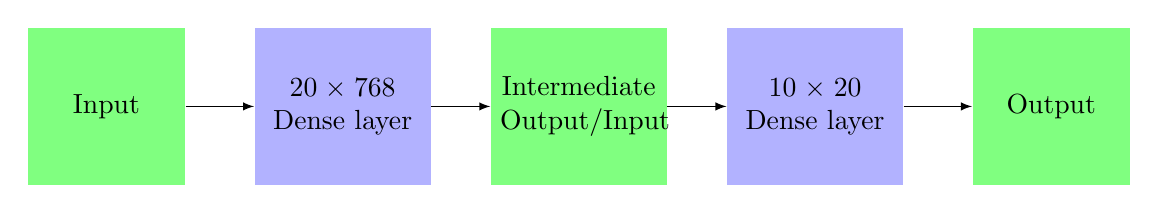
\begin{tikzpicture}[squarednode/.style={rectangle, minimum size=2cm},>=latex
	]
	\path
	+(0,0)  node[squarednode,fill=green!50]  (1) {Input}
	+(3,0)  node[text width=2cm,align=center,squarednode,fill=blue!30]  (2) {$20\times 768$\\Dense layer}
	+(6,0)  node[text width=2cm,align=center,squarednode,fill=green!50]  (3) {Intermediate\\Output/Input}
	+(9,0)  node[text width=2cm,align=center,squarednode,fill=blue!30]  (4) {$10\times 20$\\Dense layer}
	+(12,0)  node[squarednode,fill=green!50]  (5) {Output}
	;
	\draw[->] (1)--(2);
	\draw[->] (2)--(3);
	\draw[->] (3)--(4);
	\draw[->] (4)--(5);
	\end{tikzpicture}
	\caption{20 FCN for neuromorphic circuit}
	\label{fig:20fcn}
\end{figure}
\begin{figure}[H]
	\centering
	\includegraphics[scale=0.7]{predict.png}
	\caption{Prediction of last 40 handwritten digits from intermediate
		output/input
		of 10000 MNIST test data (predicted in top left corner with true in green and false in red)}
	\label{fig:predict}
\end{figure}
In previous chosen 20 FCN model for neuromorphic network implementation, we make the ReLU activation function redundant by processing the weight to $0 \geq w_c \geq 1$, and with our input $0 \geq V_{\text{in}} \geq 1$, all the outputs are naturally $>0$, which are already the same as outputs of a ReLU function even when it is implemented. Softmax function are not implemented in neuromorphic network due to the inherent complexity, so only post processing for Softmax are used.

After taking the architecture of 20 FCN, trained weights of $10\times 20$ dense layer, and intermediate output/input from $20\times 768$ dense layer (Figure \ref{fig:20fcn}) from TensorFlow and transferring it to neuromorphic network in Cadence, the simulation on Cadence was run to test the performance of off-chip learning for 1000 MNIST test dataset. OpenCV was used to visualise the last 40 samples of test dataset and their predicted values (Figure \ref{fig:predict}).

The performance for small scale $10\times 20$ dense layer was astonishing. It achieved an accuracy of $81.02\%$ vs $80.24\%$ predicted by TensorFlow. Rounding errors may be very helpful in improving network performance by chance.

Full simulation of 20 FCN was too conducted with a miserable accuracy of around $10\%$ due to the reasons in Challenges section (section \ref{sect:cha}) as all outputs are stuck at predicting 0. Basically, access to better performing opamp model is needed to pull the feat off.